\documentclass[a4paper]{ctexart}
\usepackage[top=2.3cm,bottom=2cm,left=1.7cm,right=1.7cm]{geometry} 
\usepackage{amsmath, amssymb}
\usepackage{color}
\usepackage{pythonhighlight}
\usepackage{listings}
\usepackage{mathrsfs} 
\usepackage{booktabs}
\usepackage{amsthm}
\usepackage{longtable} 
\usepackage{graphicx}
\usepackage{subfigure}
\usepackage{caption}
\usepackage{fontspec}
\usepackage{titlesec}
\usepackage{fancyhdr}
\usepackage{latexsym}
\usepackage{subfigure}
\def\d{\mathrm{d}}
\def\e{\mathrm{e}}
\def\degree{$^{\circ}$}
\title{\textbf{捕食者-被捕食者模型的简单模拟}}
\author{化学与分子工程学院\;王崇斌\;1800011716\\生命科学学院\;张芷瑄\;1800012192\\生命科学学院\;魏曈\;1800012140}
\date{}
\makeatletter %使\section中的内容左对齐
\renewcommand{\section}{\@startsection{section}{1}{0mm}
	{-\baselineskip}{0.5\baselineskip}{\bf\leftline}}
\makeatother
\begin{document}
    \pagestyle{fancy}
    \lhead{数据结构与算法}
	\chead{}
	\rhead{}
	\maketitle
	\thispagestyle{fancy}
	\section{\Large{问题背景和设计思路}}
	\subsection{\large{Lotka–Volterra模型}}
	\paragraph{}假定被捕食者食物充足,也即在没有捕食者时数量呈指数增长,而捕食者在没有被捕食者时数量指数下降。
	当两者共同存在时,假定捕食者完全以被捕食者为食且胃口无限,此时我们用$N$代表被捕食者数量,用$P$代表被捕食者数量,
	用数量,那么$N$的减少率应该依赖于两者相遇的概率和捕食者对于猎物进攻的效率,那么被捕食者地数量可以一般地表达为:
	\begin{align}
		\frac{\d N}{\d t} = (r_{1} - \epsilon P)N
	\end{align}
	其中$r_{1}$代表了被捕食者的内禀增长能力,$\epsilon$代表了捕食者发现猎物和进攻猎物的效率。
	对于捕食者,新产生捕食者的速率应与$NP$成正比,可以一般地表达为:
	\begin{align}
		\frac{\d P}{\d t} = (-r_{2} + \theta N)P
	\end{align}
	上述两个方程即是对Lotka-Volterra模型的定量描述,通常也称为Lotka-Volterra方程。
	考虑$r_{1} = 0.6,\;\epsilon=0.3,\;r_{2} = 0.2,\;\theta=0.05,\;P(0) = 10,\;N(0)=5$使用mathematica给出
	此方程组的数值解如图1所示,
	\begin{figure}[htbp]
		\centering
		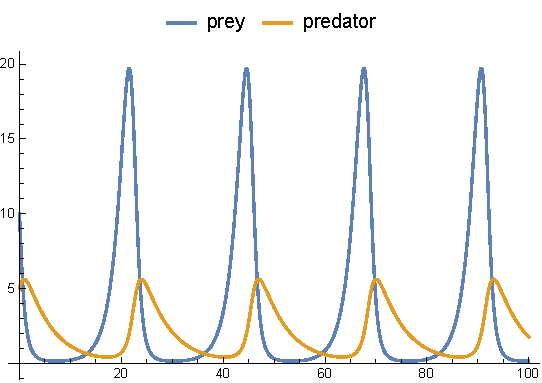
\includegraphics[scale=0.90]{lotka-volterra.pdf}
		\caption{}
	\end{figure}
	可以看出捕食者于被捕食者数量在此模型下呈现出规律的周期变化。
	\paragraph{}
	受到Lotka-Volterra模型以及高斯的基于此模型而进行的真实实验验证,我们也希望能用python程序更加准确地来模拟和可视化
	此捕食者和被捕食者系统呈现周期性振荡过程,捕食者和被捕食者的可视化繁殖过程和数量关系图,
	并试图通过改变不同的参数来改变捕食者和被捕食者的捕食和繁殖特性,对最终图形波动程度和数量关系图进行分析。
	\subsection{\large{对于Lotka–Volterra模型的改进和模拟思路}}
		\paragraph{}
		我们此时考虑一个稍微复杂的系统,其中包含一个简单的食物链:草-食草动物(被捕食者)-食肉动物(捕食者)。同时考虑
		空间有限,那么草就不能像Lotka–Volterra模型中的被捕食者一样数量指数增长,而是会受到限制。我们考虑使用$g,\;f,\;b$分别代表
		草、食草动物、食肉动物。首先考虑草的演化,考虑到种群对自身增长的阻滞与草被食草动物吃掉,用如下方程描述草的演化:
		\begin{align}
			\frac{\d g}{\d t} = k_{1}g\left(1-\frac{g}{N_{1}}\right) - k_{2}fg
		\end{align}
		考虑到食草动物本身的指数衰减、被食肉动物吃掉、吃草而数量增长(考虑自身阻滞),用下述方程来描述其演化:
		\begin{align}
			\frac{\d f}{\d t} = k_{3}gf\left(1 - \frac{f}{N_{2}}\right) - k_{4}f - k_{5}fb
		\end{align}
		考虑食肉动物因为吃食草动物而数量增长、单独存在时数量的指数衰减,给出方程:
		\begin{align}
			\frac{\d b}{\d t} = k_{6}fb\left(1 - \frac{b}{N_{3}}\right) - k_{7}b
		\end{align}
		(以上方程为作者本人提出,可能会有不合理之处)在参数$k_{1} = 2,\;N_{1} = 100,\;k_{2} = 0.3,\;k_{3} = 0.6,\;N_{2} = 70, \;k_{4} = 0.4,\;k_{5} = 0.2,\;k_{6} = 0.2,\;N_{3} = 20,\;k_{7} = 1, g(0)=20,\;f(0)=10,\;b(0)=5$下数值求解上述
		微分方程组,得到图2所示结果。
		\begin{figure}[htbp]
			\centering
			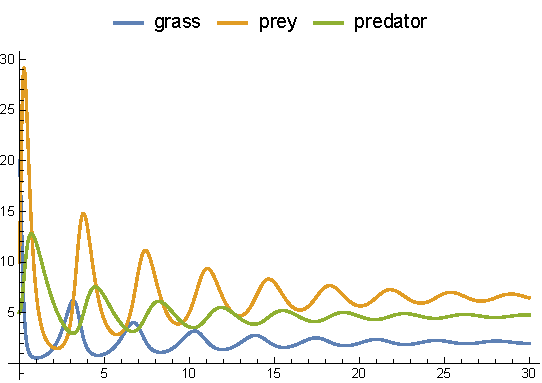
\includegraphics[scale=0.90]{mymodel.pdf}
			\caption{}
		\end{figure}
		可以看出在一定范围内三者数量呈现出良好的周期性,最后会趋于稳定。
		但是上述模型只是对于种群整体行为的模拟,我们希望通过计算机给出一个基于个体行为的种群数量模拟,这便是我们想要解决的问题。
		\paragraph{}
		在最初的代码编写时,我们设计了随机产生的不可移动可繁殖的食物和可自由移动能够和繁殖的细菌
		,也能够得到类似的图像和结果,但由于与实际情况差异较大,于是加入了草(grass)的设定。在这个模型里,
		每一个格子代表的是单位数量的种群还是独立的个体有待商榷。
		\paragraph{}
		这是一个极为简化的模型,在一块可自定义设置大小的样方地中,草:有生长能力且生长不
		可以受到限制(可以设置每格最大草的数量),有食草动物存在时减少(被吃掉)。食草动物:自由移动,饥饿会导致死亡,有寿命,
		在不饥饿时繁殖。食肉动物:自由移动,饥饿会导致死亡,有寿命,在不饥饿时繁殖。\\
		\\
	\section{\Large{主代码以及代码分析}}
	\paragraph{程序所依赖的模块}
	负责运算的程序主要依赖numpy模块来产生随机数。在可视化的部分使用tkinter模块构建图形界面,
	使用matplotlib.pyplot模块绘制了各种关系图,同时使用matplotlib.animation实现了对于实时数据
	的动态更新。
	\\
	\begin{python}
	import numpy as np
	
	
	class Bacteria():
		"""
		Bacteria类
		可以认为这是对会繁殖、会运动、有寿命、会饿死的捕食者的模拟
		"""
		__num = 0  # 记录Bacteria类中实例数量
		rp_prob = 0.9  # 记录Bacteria实例达到分裂条件时的分裂概率
		__lifetime = 40  # 记录Bacteria类实例的寿命
		__hunger = 1  # 记录Bacteria类中实例的默认饥饿值
		__tig = 5  # 记录Bacteria类中实例的分裂触发值

		def __init__(self,lifetime=40,hunger=3,tig=5):
			self.lifetime = lifetime  # bacteria寿命
			self.hunger = hunger  # 饥饿值,值越低而越饥饿,饥饿值为1而仍未找到食物则会死亡
			self.tig = tig  # 繁殖的触发条件,只有在饥饿值高于此值的时候才能繁殖
			Bacteria.__num += 1  # 当创建实例时,记录数量的__num加一
	
		def __del__(self):
			"""
			定义了实例被删除时的行为
			"""
			if Bacteria.__num >= 0:
				Bacteria.__num -= 1  # 被删除时__num减一
			else:
				raise ValueError("Bacteria.__del__()类中没有实例")
	
		def can_divide(self):
			return self.hunger > self.tig# 表示捕食者能够进行繁殖的最低饥饿值条件
	
		@classmethod
		def get_num(cls):
			return Bacteria.__num
		
		@classmethod
		def set_lifetime(cls, lifetime):
			"""设置寿命"""
			Bacteria.__lifetime = lifetime
	
		@classmethod
		def set_hunger(cls, hunger):
			"""设置饥饿值"""
			Bacteria.__hunger = hunger
	
		@classmethod
		def set_tig(cls, tig):
			"""设置分裂触发值"""
			Bacteria.__tig = tig
	
	class Food():
		"""
		food类
		考虑food是一种会运动、会繁殖的被捕食者,会吃草,有饥饿值
		"""
		__num = 0  # 记录Food实例数量
		rp_prob = 0.6  # 记录Food类实例的繁殖概率
		__lifetime = 20  # 记录Food类实例的寿命
		__hunger = 1  # 记录Food类实例的饥饿值
		__tig = 2  # 记录Food实例的繁殖触发值
	
		def __init__(self, lifetime=20, hunger=5, tig=1):
			Food.__num += 1
			self.hunger = hunger
			self.tig = tig  # food繁殖的触发条件,一般考虑food繁殖能力强,此值默认比较小
			self.lifetime = lifetime  # Food实例的寿命
	
		def __del__(self):
			if Food.__num >= 0:
				Food.__num -= 1
			else:
				raise ValueError("Food.__del__()类中没有实例")
	
		def can_divide(self):
			return self.hunger > self.tig# 表示被捕食者能够进行繁殖的最低饥饿值条件
	
		@classmethod
		def get_num(cls):
			return Food.__num
	
		@classmethod
		def set_lifetime(cls, lifetime):
			Food.__lifetime = lifetime
	
		@classmethod
		def set_hunger(cls, hunger):
			Food.__hunger = hunger
	
		@classmethod
		def set_tig(cls, tig):
			Food.__tig = tig

	class Field():
		"""
		表示一块可供bacteria活动的区域,要求此类有且仅有一个实例
		"""
		# 以下参数的设置都在类方法中完成
		__grass_growth_list = []  # 记录“草”的增长模式,二维列表,每一格存储“草”的增长速率
		# 希望可以设计出除了平均分布以外的分布
		__average_rate = 0  # 记录平均增长时增长速率
		size = 0
		__food_num = []  # 记录每次更新之后food的数量
		__bacteria_num = []  # 记录每次更新之后bacteria的数量
		__direction = {
			0: (0, 1),
			1: (-1, 1),
			2: (-1, 0),
			3: (-1, -1),
			4: (0, -1),
			5: (1, -1),
			6: (1, 0),
			7: (1, 1)
		}# food 和 bacteria可能的移动方向,不包括留在原地的选项,因此后续代码要注意加上这种可能性
		def __init__(self, n, mode="plain", grass_i=5):
			"""
			n: 区域大小,表示这是一个(n, n)的区域
	
			考虑了food和bacteria都有运动能力并且可以繁殖
			food要依靠吃“草”来生活,预设每格草的量为5
			在初始化时更新所有的类变量
	
			期待着通过mode这个参数调节food的分布规律
			"""
			Field.clear_bacteria_num()
			Field.clear_food_num()
			Field.set_average_rate()
			self.__size = n
			Field.size = n
			self.__state = [[None for i in range(n)] for i in range(n)]  # 初始化构造空区域
			# 需要调用set_food与set_bacteria向区域中加入food和bacteria
			if mode == "plain":
				# 设置草的分布规律,草另行储存
				Field.plain_mode()  # 这个构造了草的增长速率列表
				self.__grass = [[grass_i for i in range(n)] for j in range(n)]
				# grass是food的food,此属性储存了当前区域grass数量分布
	
		def __str__(self):
			"""
			调试的时候用一用
			"""
			return str(self.transform())
	
		def set_bacteria(self, coordinate=(0, 0)):
			"""
			设置bacteria初始位置,每次执行只能设置一个bacteria的位置
			"""
			i, j = coordinate
			if i >= self.__size or j >= self.__size:
				raise IndexError("Field.set_bacteria()设置位置超过了区域大小")
	
			old = self.__state[i][j]
			self.__state[i][j] = Bacteria()
			del old
	
		def set_food(self, coordinate):
			"""
			设置food初始位置,每次执行只能设置一个food位置
			"""
			i, j = coordinate
			if i >= self.__size or j >= self.__size:
				raise IndexError("Field.set_food()设置位置超过了区域大小")
			old = self.__state[i][j]
			self.__state[i][j] = Food()
			del old
	
		def evolution(self, coordinate):
			"""
			选取区域中的一个位置coordinate,分析这里可能发生的情况
			分为三类,food、bacteria、空地
			注意只要是food没有吃grass,grass就会增加
			"""
			i, j = coordinate[0], coordinate[1]
			if i >= self.__size or j >= self.__size:
				raise IndexError("Field.evolution()选取位置超过区域大小")
	
			old = self.__state[i][j]  # 取出i, j位置的对象的引用
	
			if isinstance(old, Food):  # 如果是food
				empty_pos = []  # 储存附近有grass的空地,表示这是food可以去的空地
				food_pos = []  # 储存附近的food
				for d in range(8):
					direction = Field.__direction[d]
					position = i + direction[0], j + direction[1] # 周围所有的八个位置
					if not Field.out_of_range(Field.size, position): 
						sur = self.__state[position[0]][position[1]]
						if sur is None:
							if self.__grass[position[0]][position[1]] > 0:
								empty_pos.append(position) # 如果这个位置是有grass且没有food和bacteria的,则作为一个可去的位置存储下来
						elif isinstance(sur, Food):
							food_pos.append(position)
				if self.__grass[i][j] > 0:
					empty_pos.append(coordinate)  # food有可能不动
	
				def move_food(old):
					"""描述food在不分裂时的行为,假设food所在的地方grass不生长
					同时假设food只会向有grass的地方前进"""
					old.lifetime -= 1  # 寿命减1
					if empty_pos == []:  # 表示周围所有地方的草都没有了,待在原地
						if self.__grass[i][j] == 0:
							old.hunger -= 1  # 如果被捕食者所处位置没有草,饥饿值减一
						else:
							self.__grass[i][j] -= 1
					else:
						index = np.random.randint(len(empty_pos))  # 随机选取一个可行的方向
						nxt_pos = empty_pos[index]  # 表示food下一步前进的位置
						self.__state[i][j] = None
						self.__state[nxt_pos[0]][nxt_pos[1]] = old
						self.__grass[nxt_pos[0]][
							nxt_pos[1]] -= 1  # 表示前去的那个地方grass被吃掉1
						old.hunger += 1
	
				if old.lifetime == 1:
					self.__state[i][j] = None
					del old  # 删除food的引用,Food类中记录实例数量的变量减1
					self.grass_grow(coordinate)  # 没有food后,grass会生长
				elif old.hunger == 1:  # 如果饥饿值为1,要吃grass
					if empty_pos == []:  # 表示周围没有空位,此时被饿死
						self.__state[i][j] = None
						del old
					else:
						move_food(old)
				elif old.hunger > 1:  # 饥饿值大于1,考虑分裂或者向其他方向运动,但都会吃grass
					if old.hunger > old.tig:  # 说明达到了分裂条件,有概率分裂
						positions = empty_pos[:-1]  # 除了当前位置的有grass的所有相邻位置
						if len(positions) == 0:  # 没有空间支持food繁殖,则不分裂,可能向有grass的位置移动
							move_food(old)
						else:
							r = np.random.random_sample()
							if r < Food.rp_prob:  # 此时表示可以繁殖,向周围任意有grass空地繁殖而自己本身不移动
								old.hunger -= 1
								idx = np.random.randint(len(positions))
								new_pos = positions[idx]
								self.__state[new_pos[0]][new_pos[1]] = Food()
								# 繁殖结果为一个饥饿值为初始值,寿命为初始值的food
								self.__grass[new_pos[0]][new_pos[1]] -= 1
							else:
								move_food(old)
					else:  # 未达到分裂条件,只能考虑运动,注意只能向没有Bacteria的地方运动
						move_food(old)
			elif isinstance(old, Bacteria):
				# 如果是bacteria,考虑向周围运动,同时也要考虑bacteria的死亡情况
				empty_pos = []  # 表示空位的位置
				food_pos = []  # 表示food的位置
				for x in range(8):  # 注意i, j已经用过了
					direction = Field.__direction[x]
					position = i + direction[0], j + direction[1]
					if not Field.out_of_range(Field.size, position):
						sur = self.__state[position[0]][position[1]]
						# 分析周围环境
						if isinstance(sur, Food):
							food_pos.append(position)
						elif isinstance(sur, Bacteria):
							continue
						elif sur is None:
							empty_pos.append(position)
						else:
							raise Exception("Field.evolution()未知错误")
	
				def move_bacteria(old):
					"""描述了bacteria不分裂时的行为"""
					num_food = len(food_pos)
					num_empty = len(empty_pos)
					move_prob = (num_empty + 1) / (num_empty + num_food + 1) # 不移动的可能性是没有food的位置和原地比上总共九个位置
					r = np.random.random_sample()
					if food_pos != [] and r > move_prob:  # 如果周围有food,吃掉食物且向有food的位置随机前进
						old.hunger += 1
						nxt_pos = food_pos[np.random.randint(len(food_pos))]
						food = self.__state[nxt_pos[0]][nxt_pos[1]]
						self.__state[i][j] = None
						self.__state[nxt_pos[0]][nxt_pos[1]] = old
						del food
					else:
						old.hunger -= 1  # 如果周围没有food留在原地或者移动,变得更加饥饿
						empty = [(i, j)] + empty_pos
						nxt_pos = empty[np.random.randint(len(empty))]
						self.__state[i][j] = None
						self.__state[nxt_pos[0]][nxt_pos[1]] = old
	
				# 下面要讨论bacteria面对空位和food的具体选择问题,这时候会包含bacteria的繁殖
				if old.lifetime == 1:
					self.__state[i][j] = None
					del old
				else:
					old.lifetime -= 1  # 如果寿命不是1,寿命减一
					if old.hunger == 1:  # 讨论饥饿值
						# 首先是饥饿值仅剩1的情况
						if food_pos == []:  # 周围没有food,会被饿死
							self.__state[i][j] = None
							del old
						else:
							nxt = food_pos[np.random.randint(
								len(food_pos))]  # 随机挑选一个位置
							food = self.__state[nxt[0]][nxt[1]]
							old.hunger += 1
							self.__state[nxt[0]][nxt[1]] = old
							# 将被选中food所占的位置替换为原来的bacteria
							self.__state[i][j] = None
							del food  # 删除被吃food的引用,food总数减一
					elif old.hunger > old.tig:
						# 当饥饿值大于设定值,触发分裂条件,有一定概率分裂
						r = np.random.random_sample()
						if r < Bacteria.rp_prob and empty_pos != []:  # 判断是否分裂
							new_bac = Bacteria()  # 认为新生成的Bacteria饥饿值为初始的设定值
							old.hunger -= 1  # 繁殖需要消耗饥饿值
							new_pos = empty_pos[np.random.randint(len(empty_pos))]
							self.__state[new_pos[0]][new_pos[1]] = new_bac
						else:
							move_bacteria(old)
					else:
						# 剩余的情况,只有向空位移动或者吃food
						move_bacteria(old)
			elif old is None:
				# 如果是空地,我们只考虑grass增长
				self.grass_grow(coordinate)
			else:
				raise Exception("Field.evolution()未知错误")
	
		def transform(self):
			"""
			将self.__state的数据转化为容易观察的数据
			food用0代表,bacteria用1代表
			"""
			list_output = [[] for i in range(Field.size)]
			for x in range(Field.size):
				for y in range(Field.size):
					now = self.__state[x][y]
					if isinstance(now, Food):
						list_output[x].append(0)
					elif isinstance(now, Bacteria):
						list_output[x].append(1)
					elif now is None:
						list_output[x].append(None)
			return list_output
	
		def update(self):
			"""
			执行一次算作对于状态的一次更新,返回一个由0,1,None组成的二维列表
			"""
			cnt = 0
			while cnt < Field.size**2:
				i, j = np.random.randint(0, Field.size), np.random.randint(
					0, Field.size)
				self.evolution((i, j))
				cnt += 1
			Field.__bacteria_num.append(Bacteria.get_num())
			Field.__food_num.append(Food.get_num())
			return self.transform()
	
		def grass_grow(self, coordinate, max=5):
			"""描述一个位置草的生长,写成函数用起来方便嘛"""
			i, j = coordinate
			if i >= self.__size or j >= self.__size:
				raise IndexError("Field.grass_grow()所选位置超出了区域范围")
			if self.__grass[i][j] < 9:
				self.__grass[i][j] += self.__grass_growth_list[i][j]
	
		def get_grass(self):
			"""调试的时候用一用"""
			return self.__grass
	
		@staticmethod
		def out_of_range(size, pos):
			if (pos[0] < size and pos[0] >= 0) and (pos[1] < size and pos[1] >= 0):
				return False
			else:
				return True
	
		@classmethod
		def plain_mode(cls):  # 我的梦想是可以让草的增长实现一定的分布规律
			"""平均增长列表的构造,注意要先调用set_average_rate()与设置size"""
			Field.__grass_growth_list = [[
				Field.__average_rate for i in range(Field.size)
			] for i in range(Field.size)]
	
		@classmethod
		def set_average_rate(cls, rate=1):
			Field.__average_rate = rate
	
		@classmethod
		def clear_food_num(cls):
			Field.__food_num = []
	
		@classmethod
		def get_food_num_list(cls):
			return Field.__food_num
	
		@classmethod
		def clear_bacteria_num(cls):
			Field.__bacteria_num = []
	
		@classmethod
		def get_bacteria_num_list(cls):
			return Field.__bacteria_num
	
		@classmethod
		def get_grass_growth_list(cls):
			return Field.__grass_growth_list
	\end{python}
	\begin{align*}
		\quad
	\end{align*}
	\section{\Large{程序使用说明}}
		\paragraph{参数设置:}
		在使用时可自由设置的参数有,图像大小,用于自定义生成一个n*n大小的图像,捕食者寿命和和被捕食者寿命均代表在程序中被选中相应次数后就会死亡
		,捕食者和被捕食者的默认饥饿值是初始生成时或繁殖产生新捕食者或被捕食者的饥饿值,当捕食者和被捕食者获得食物时,饥饿值加一,否则减一,当饥饿值降为0时,会死亡。
		捕食者和被捕食者饥饿触发值,是指仅当饥饿值大于此值时,分裂才有可能进行,此值设置越高,则分裂越不容易发生;二者的繁殖概率均指二者到达触发条件后繁殖发生的概率,概率越高,繁殖能力越强。
		更新次数可以自定义设置。
		\begin{figure}[htbp]
			\centering
			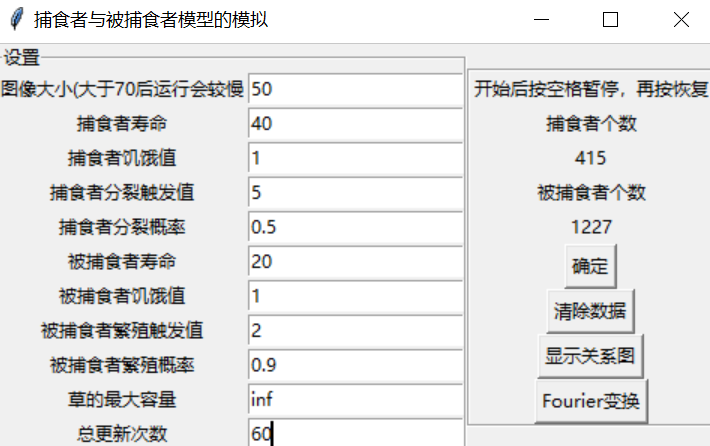
\includegraphics[scale=0.40]{mainwindow.png}
			\caption{图形界面的窗口}
		\end{figure}
		\paragraph{运行:}
		设置好参数后点击界面上的“确定”按钮程序开始运行。
		运行时,实时显示捕食者和被捕食者数量,实时显示捕食者和被捕食者在样方中的分布,捕食者数量/被捕食者数量-更新次数图像实时描绘,按空格键可控制暂停和继续。
		将光标移到曲线上,可以看到曲线上每个点对应的x,y值。
		想要终止程序只需要点击matplotlib界面的关闭按钮,这时数据会被保存下来,可以点击“显示关系图”按钮保存并查看捕食者
		与被捕食者数量随时间的演化关系图。如果点击“清除数据”,那么上一次运行的结果会被清除,可以进行下一次模拟。\\
		\\
		\\
	\section{\Large{运行结果分析}}
	\paragraph{0.}首先必须说明,并不是所有可以选择的参数组合都对应于实际情况。同时由于程序中的所有过程都是通过随机数
	决定的,不能保证同一组参数多次重复得到完全相同的结果。
	\paragraph{1.}
	参数设置为50*50大小,捕食者寿命20,饥饿值1,繁殖触发值3,繁殖概率0.6,被捕食者寿命20,饥饿值1,繁殖触发值为2,繁殖概率0.7,
	不限制草的最大数量。
	可以看出图像具有一定的周期性。参见图1:
	\begin{figure}[htbp]
		\centering
		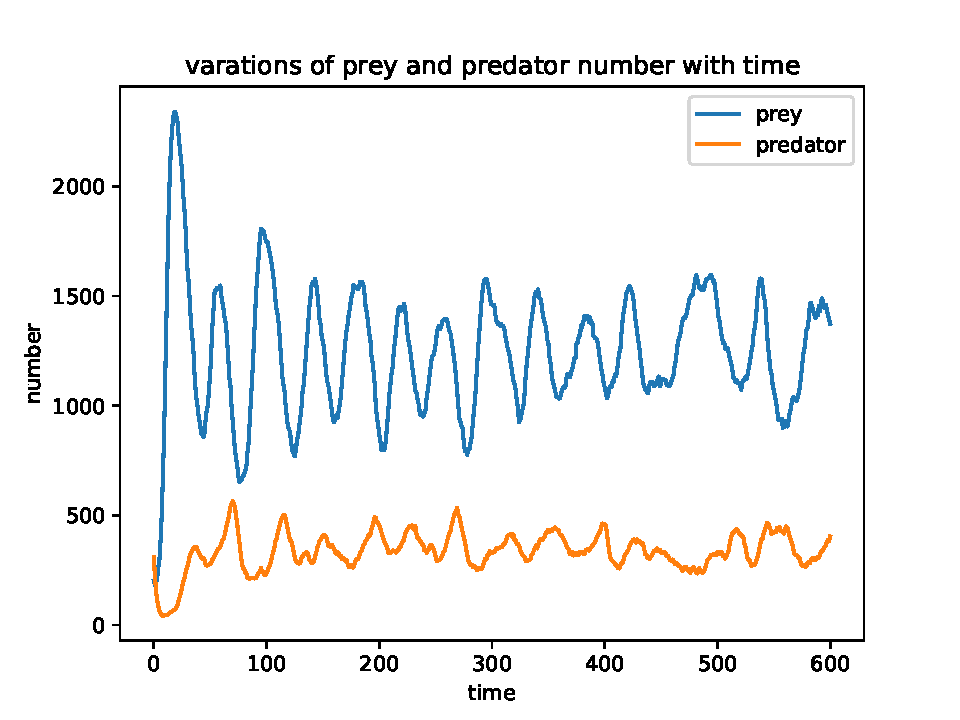
\includegraphics[scale=0.6]{demo1.pdf}
		\caption{}
	\end{figure}
	\paragraph{2.}
	参数设置为70*70大小,捕食者寿命20,默认饥饿值为1,繁殖触发值为3,繁殖概率为0.6;被捕食者寿命为20,默认饥饿值为1,繁殖概率为0.7,不限制草的数量,
	设置被捕食者繁殖触发值为2和4,可以看出当捕食者数量波动较大时,被捕食者的数量
	也会有明显的波动,这说明捕食者与被捕食者的数量变化幅度呈现出正相关,这与我们对于现实中的捕食者与被捕食者
	的认识是相同的:捕食者数量的增加导致被捕食者数量急剧下降,此后捕食者因为食物短缺而饿死,数量下降,被捕食者的
	数量会反弹。当被捕食者繁殖触发值上升时,被捕食者的繁殖能力下降,可以看出两个物种的数量变化幅度均下降。(图5的(a)和(b))
	\begin{figure}[htbp]
		\centering
		\subfigure[触发值=2]{
		\begin{minipage}{0.48\linewidth}
		\centering
		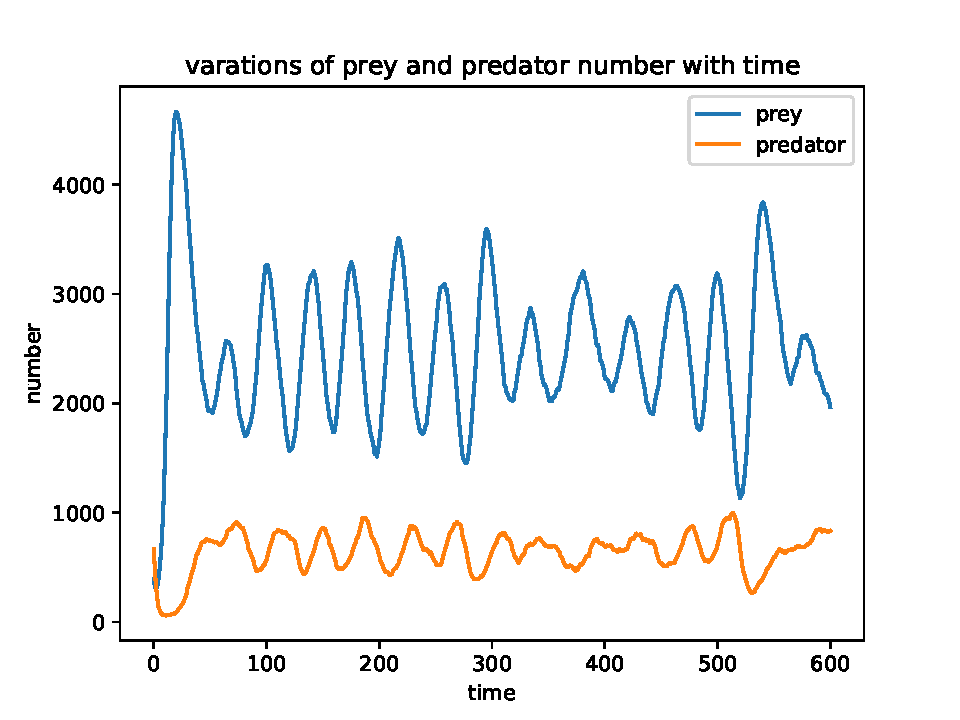
\includegraphics[scale=0.57]{demo2.pdf}
		\end{minipage}
		}%
		\subfigure[触发值=4]{
		\begin{minipage}{0.48\linewidth}
		\centering
		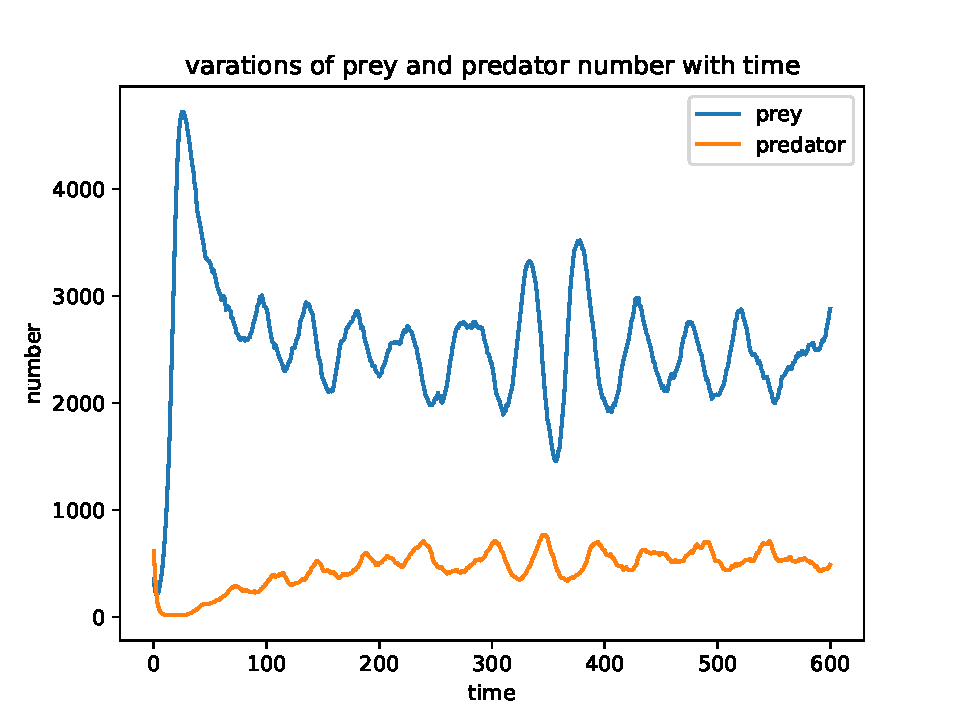
\includegraphics[scale=0.57]{demo3.pdf}
		\end{minipage}
		}%
		\caption{改变捕食者繁殖触发值对于系统的影响}
		\label{tigvalue}
	\end{figure}
	\paragraph{3.}设置图像大小为50*50,捕食者寿命为40,默认饥饿值为1,繁殖触发值3,繁殖概率0.8;
	被捕食者寿命20,默认饥饿值1,繁殖触发值2,繁殖概率0.9;草的最大容量不限制。运行后得到比较精细的
	捕食者被捕食者数量关系图(图6),捕食者的数量极大值总是先于被捕食者的数量极小值的到来(有相位差)。
	\begin{figure}[htbp]
		\centering
		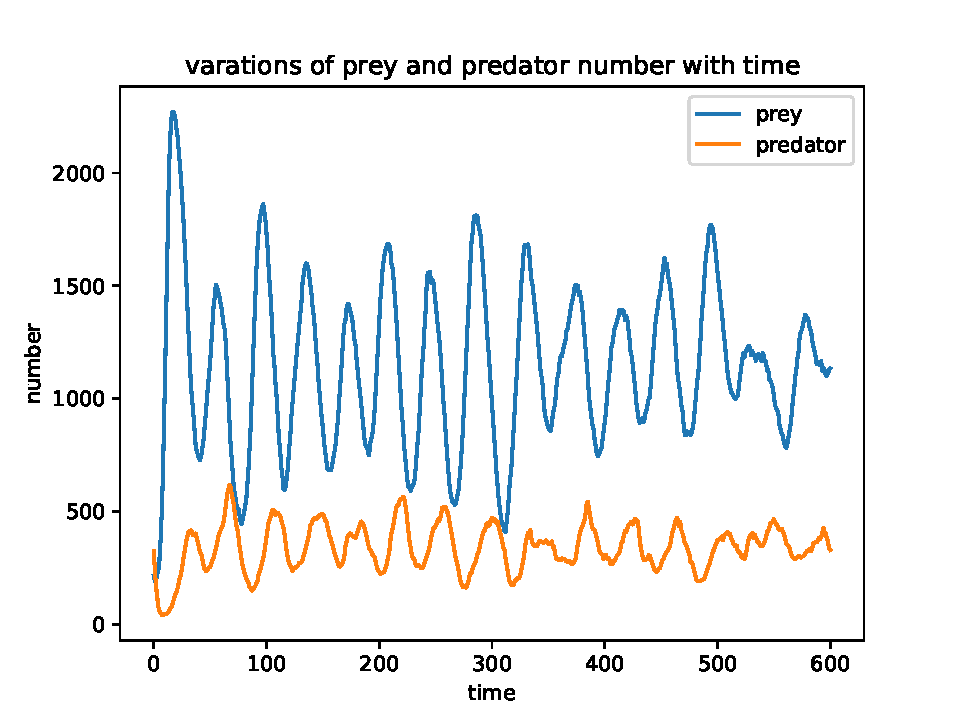
\includegraphics[scale=0.7]{demo4.pdf}
		\caption{}
	\end{figure}
	\paragraph{4.}改变被捕食者的繁殖概率对于模拟的影响
	\subparagraph{1}减小被捕食者的繁殖概率,对应于真实的情况就是被捕食者的繁殖能力下降。可以想象
	这会导致被捕食者种群数量较大的波动(因为被捕食后种群数量恢复较慢,尤其会受到捕食者数量变化的影响),同时由于被捕食者繁殖能力下降,使得
	捕食者数量维持在比较低的水平,在(3)的基础上设置参数,调整参数捕食者繁殖概率0.9,被捕食者繁殖概率0.2,进行模拟,得到
	如图7所示的结果,可以看出捕食者数量很小的波动会导致被捕食者数量较大的波动,这是因为被捕食者比较“脆弱”。
	\begin{figure}[htbp]
		\centering
		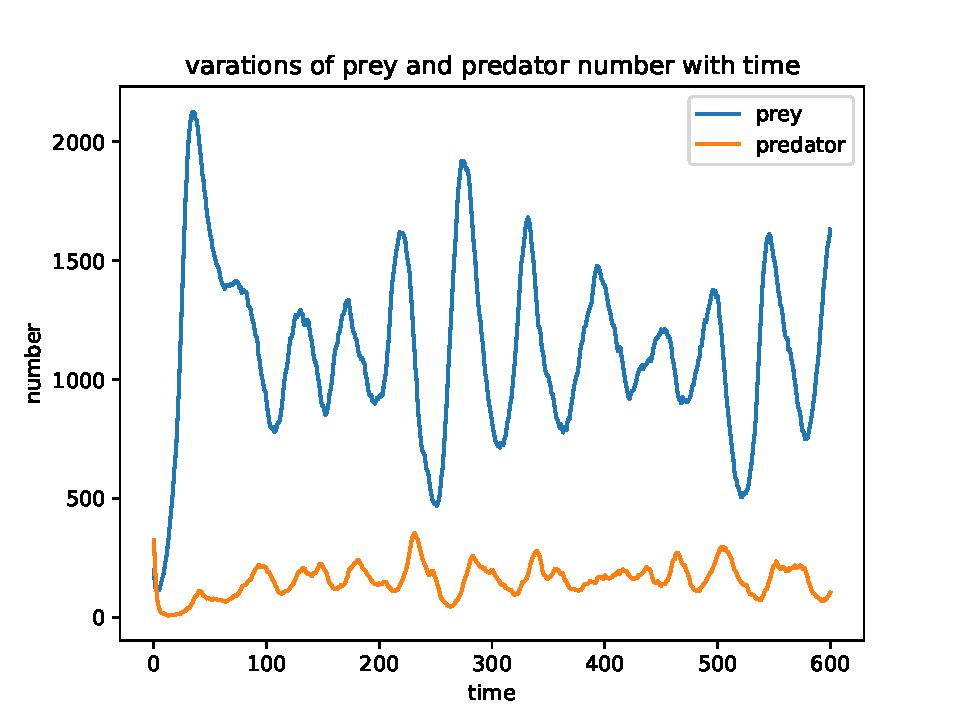
\includegraphics[scale=0.60]{demo5.pdf}
		\caption{}
	\end{figure}
	\subparagraph{2}增大被捕食者的繁殖概率,调整参数捕食者繁殖概率为0.9,被捕食者繁殖概率为1.0,进行模拟,得到如
	图8所示结果,从中可以看出,数量变化的周期性变差。
	\begin{figure}[htbp]
		\centering
		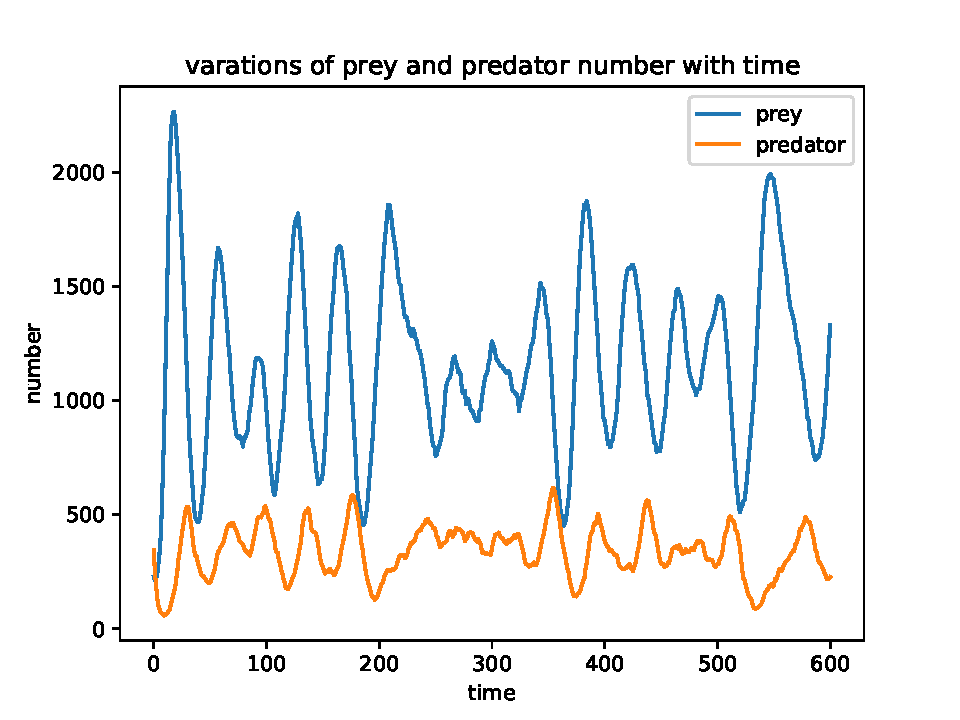
\includegraphics[scale=0.60]{demo6.pdf}
		\caption{}
	\end{figure}
	\paragraph{5}改变捕食者繁殖概率对于模拟的影响
	\subparagraph{1}
	减小捕食者的繁殖概率,可以想象捕食者的数量会趋于稳定(波动减小),且维持在一个较低的水平,同时被捕食者的数量也会相对稳定。
	设置与(3)相同的参数,将捕食者的繁殖概率改为0.05,得到如图9所示的结果,没有明显的周期性。其实可以继续降低捕食者繁殖概率,太低时捕食者种群将无法维持数量。
	\begin{figure}[htbp]
		\centering 
		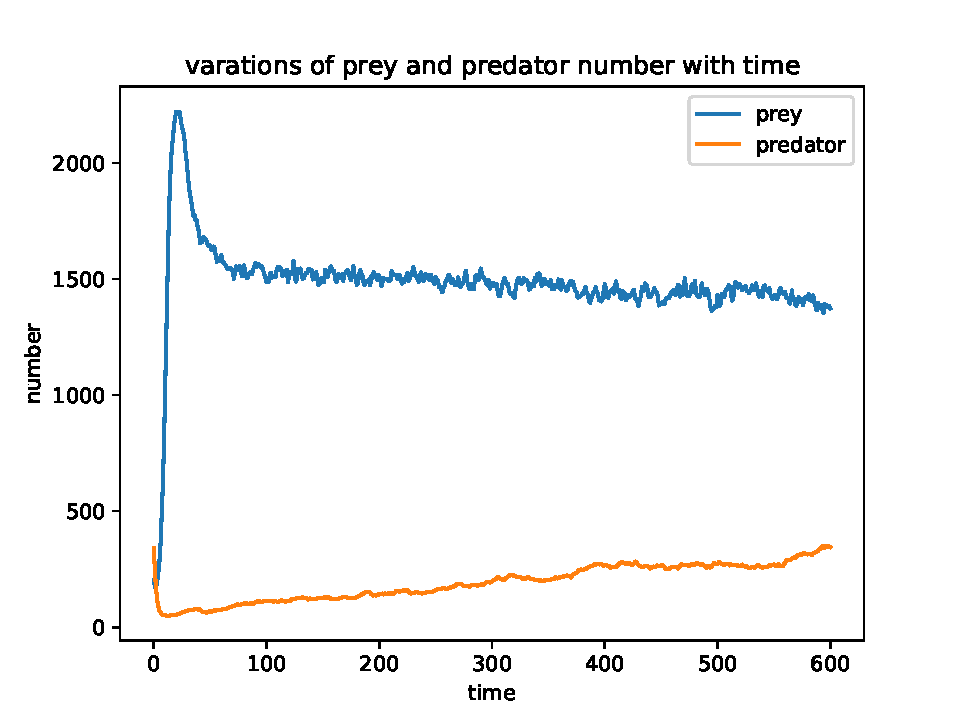
\includegraphics[scale=0.6]{demo7.pdf}
		\caption{}
	\end{figure}
	\subparagraph{2}
	略微增大捕食者的繁殖概率,在前一步的基础上将概率改为0.08,可以看出数量呈现不明显的周期性:
	\begin{figure}[htpb]
		\centering
		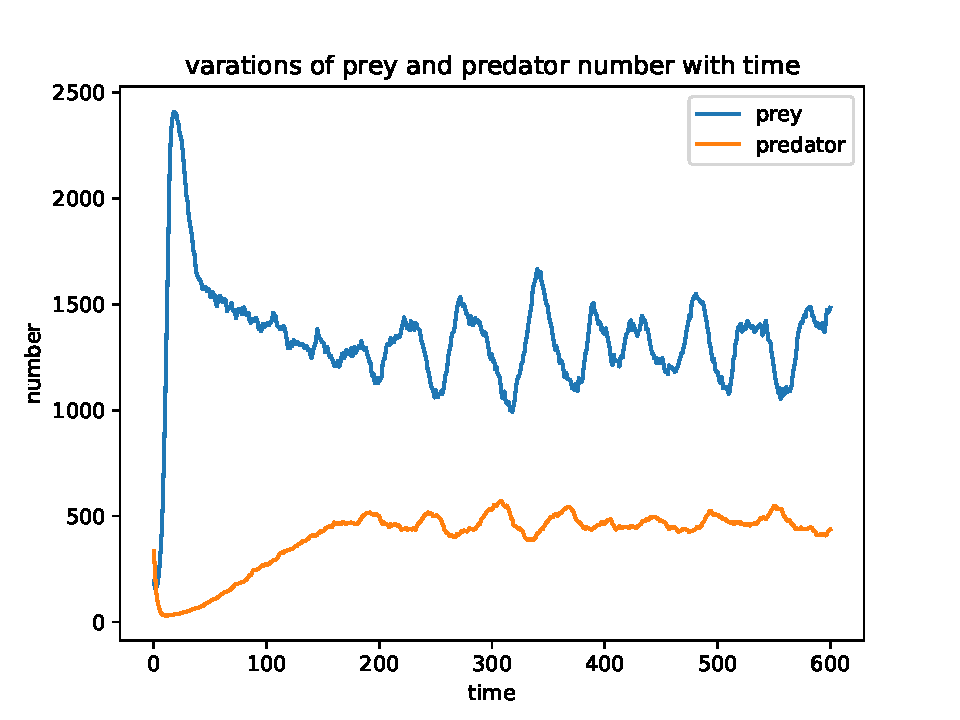
\includegraphics[scale=0.6]{demo8.pdf}
		\caption{}
	\end{figure}
	与(3)中的图7进行对比,可以看出只有当捕食者繁殖概率足够高时才能呈现出明显的周期性。同时,由于捕食者繁殖能力下降
	,导致恢复力变弱,可以从图中看到达到平衡的时间明显增长。
	\paragraph{6.}考虑场地大小对于数量变化得影响,这里采用与(3)相同的参数,只不过将场地改为100*100大小,
	运行结果如图11所示。可以与图4对比看出,当场地增大后(种群数量上升),捕食者和被捕食者的种群数量相对波动
	明显减小。这与实际情况是一致的,大的种群往往数量稳定,而小种群数量波动明显,容易灭绝(可以将场地调小,确实容易
	出现捕食者灭绝的情况)。
	\begin{figure}[htbp]
		\centering 
		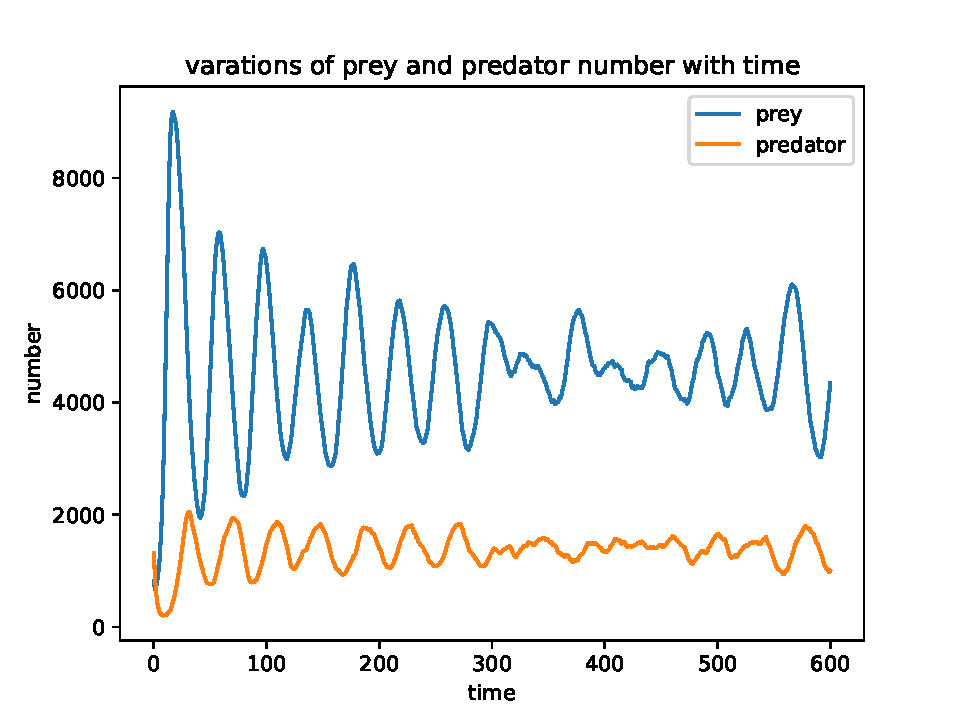
\includegraphics[scale=0.6]{demo10.pdf}
		\caption{}
	\end{figure}
	\paragraph{6.}改变捕食者繁殖触发值对于结果的影响
	\subparagraph{1}减小捕食者的繁殖触发值,在(3)的基础上,将捕食者的繁殖触发值改为1,运行结果如图12所示。
	可以看出由于调低了捕食者繁殖的触发值,繁殖速率更快了,因此也带来了较大的无规律的种群数量波动。(仔细观察两个物种的
	空间分布,可以看到规则的,奇妙的图形,就好像捕食者追着被捕食者跑一样)
	\begin{figure}[htbp]
		\centering
		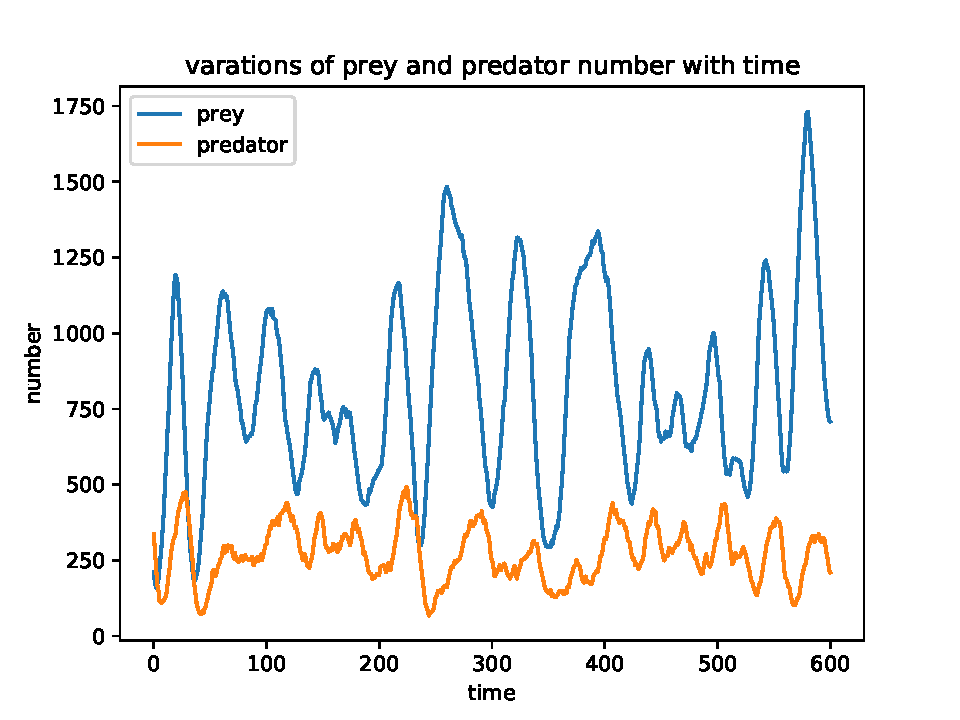
\includegraphics[scale=0.6]{demo11.pdf}
		\caption{}
	\end{figure}
	\subparagraph{2}增大捕食者的繁殖触发值,在(3)的基础上,将捕食者的繁殖触发值改为8,运行结果如图13所示。
	\begin{figure}[htbp]
		\centering 
		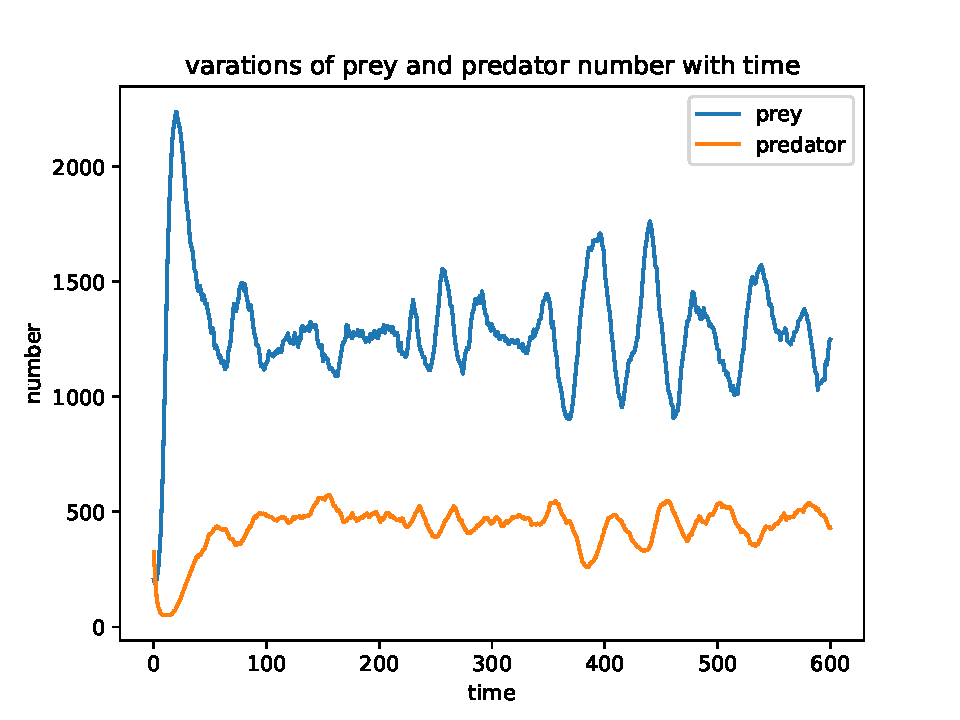
\includegraphics[scale=0.6]{demo12.pdf}
		\caption{}
	\end{figure}\\
	\\
	\section{\Large{优化方向}}
	\paragraph{}
	程序基本上实现了我们的想法,但是其中还有一些比较明显的缺陷和可以改进的地方。
	\subsection{\large{程序目前存在的缺陷}}
	\paragraph{1.}在模拟中按空格键暂停,暂停时图像会消失。
	\paragraph{2.}无法显示“草”的数量随时间的变化关系
	\paragraph{3.}动态显示的横坐标不能动态变化,当要进行短时间或者长时间观察时很不方便。
	\subsection{\large{程序可能改进的方向}}
	\paragraph{1.}在此程序中,“草”的生成是完全随机的,也就是说在空间中均匀分布,这与实际情况不一定接近,可以考虑在在不同位置对“草”
	设置不同的繁殖概率,以此实现“草”的多中心分布,进一步观察被捕食者是否会有相应的多中心分布。借此观察食物分布的不均衡对于种群数量
	和分布的影响。
	\paragraph{2.}此程序中捕食者和被捕食者的运动能力和搜寻猎物的能力非常有限,可以考虑加强它们的运动能力和搜索食物的能力。
	\paragraph{3.}可以考虑加入更多的相互竞争的物种。
	\paragraph{4.}考虑可以在程序暂停后改变参数,这样更容易对比出不同参数对于系统的影响。\\
	\\
	\\
	\section{\Large{致谢}}
	\paragraph{}
	首先感谢广大网友,没有他们在博客上无私分享自己写程序时的精彩操作与失败经历,我们也不可能在短暂的时间里获得经验与教训从而比较
	顺利地实现自己的想法,同时也感谢老师和助教耐心地解答我们关于大作业的问题。
	\paragraph{}
	感谢为了完成这个项目所辛苦付出三位同学,他们分别是来自化院的王崇斌(手机号:15388676506;邮箱:1800011716@pku.edu.cn)、来自生科的张芷瑄(手机号:18602933184;邮箱:1800012192@pku.edu.cn)
	和魏瞳(手机号:15032592997;邮箱:1800012140@pku.edu.cn)。其中王崇斌负责完成主程序的构思和
	编写和报告的排版,张芷瑄负责图形界面的设计和编写同时还有关于捕食者-被捕食者模型背景的调查,魏曈负责完善代码的注释、提高可读性,同时负责报告的撰写。
	由于不同同学完成的工作性质差异明显,我们在这里并不给出贡献排名。
\end{document}